\subsection{UC2 - Visualizza impostazioni}
\begin{figure}[H]
    \centering
    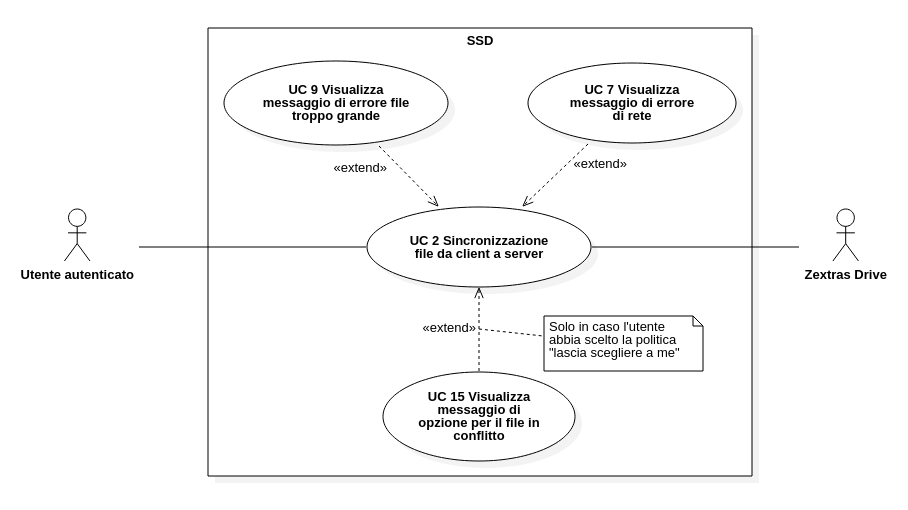
\includegraphics[scale = 0.7]{components/img/UC2.png}
    \caption{UC2 - Visualizza impostazioni}
\end{figure}
\begin{itemize}
\item \textbf{Attore Primario:} Utente autenticato;
\item \textbf{Precondizione:} L'utente vuole visualizzare le impostazioni dell'applicazione;
\item \textbf{Postcondizione:} L'utente può scegliere che impostazioni modificare;
\item \textbf{Scenario principale:}
    \begin{enumerate}
    \item L'utente entra nelle impostazioni;
    \item L'utente può vedere cosa può cambiare all'interno dell'applicazione.
    \end{enumerate}
\end{itemize}

\subsubsection{UC2.1 - Seleziona file da sincronizzare dal client al server}
\begin{figure}[H]
    \centering
    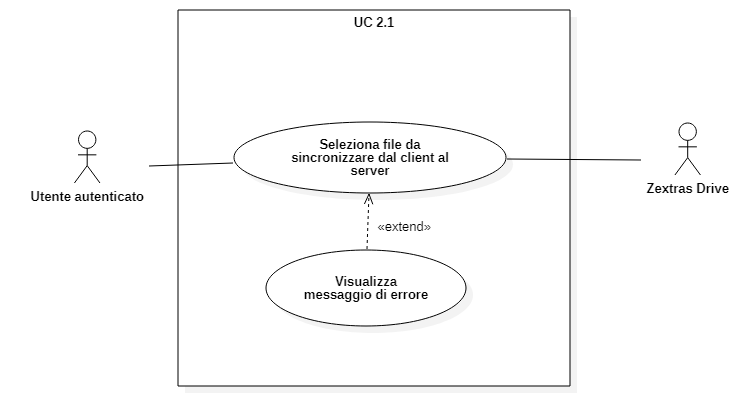
\includegraphics[scale = 0.6]{components/img/UC2_1.png}
    \caption{UC2.1 - Seleziona file da sincronizzare dal client al server}
\end{figure}
\begin{itemize}
\item \textbf{Attore Primario:} Utente autenticato;
\item \textbf{Attore Secondario:} Zextras Drive;
\item \textbf{Precondizione:} L'utente non ha selezionato nessun file da sincronizzare con il server;
\item \textbf{Postcondizione:} L'utente ha aggiunto dei file che verranno sincronizzati con il server;
\item \textbf{Scenario principale:}
    \begin{enumerate}
    \item L'utente sceglie di aggiungere dei file da sincronizzare con il server;
    \item L'utente aggiunge i file che vuole sincronizzare ad una lista presente nell'applicazione.
    \end{enumerate}
\item \textbf{Estensioni:}
    \begin{itemize}
    \item Visualizzazione messaggio di errore di rete (UC5 \S{}\ref{UC5});
    \item Visualizzazione messaggio di errore file troppo grande (UC6 \S{}\ref{UC6});
    \end{itemize}
\end{itemize}

\subsubsection{UC2.2 - Seleziona file da sincronizzare dal server al client}
\begin{figure}[H]
    \centering
    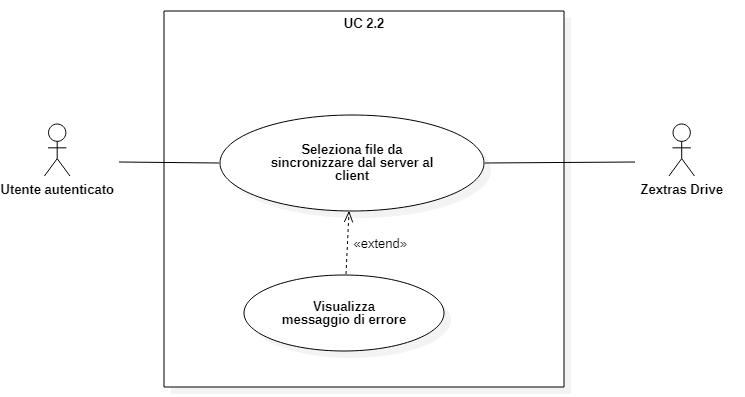
\includegraphics[scale = 0.6]{components/img/UC2_2.png}
    \caption{UC2.2 - Seleziona file da sincronizzare dal server al client}
\end{figure}
\begin{itemize}
\item \textbf{Attore Primario:} Utente autenticato;
\item \textbf{Attore Secondario:} Zextras Drive;
\item \textbf{Precondizione:} L'utente non ha selezionato nessun file da sincronizzare con il client;
\item \textbf{Postcondizione:} L'utente ha aggiunto dei file che verranno sincronizzati con il client;
\item \textbf{Scenario principale:}
    \begin{enumerate}
    \item L'utente sceglie di aggiungere dei file da sincronizzare con il client;
    \item L'utente aggiunge i file che vuole sincronizzare con il client da una lista presente nell'applicazione.
    \end{enumerate}
\item \textbf{Estensioni:}
    \begin{itemize}
    \item Visualizzazione messaggio di errore di rete (UC5 \S{}\ref{UC5});
    \item Visualizzazione messaggio di errore spazio non disponibile in locale (UC7 \S{}\ref{UC7});
    \end{itemize}
\end{itemize}

\subsubsection{UC2.3 - Seleziona quota disco}
\begin{figure}[H]
    \centering
    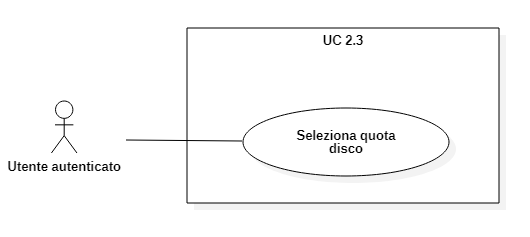
\includegraphics[scale = 0.7]{components/img/UC2_3.png}
    \caption{UC2.3 - Seleziona quota disco}
\end{figure}
\begin{itemize}
\item \textbf{Attore Primario:} Utente autenticato;
\item \textbf{Precondizione:} L'utente vuole cambiare la dimensione dei file che l'applicazione scaricherà dal server;
\item \textbf{Postcondizione:} L'utente ha deciso che file superiori al limite imposto non verranno scaricati;
\item \textbf{Scenario principale:}
    \begin{enumerate}
    \item L'utente ha poco spazio all'interno del computer;
    \item L'utente decide di inserire un filtro che limita l'applicazione da scaricare file troppo grandi.
    \end{enumerate}
\end{itemize}

\subsubsection{UC2.4 - Logout}
\begin{figure}[H]
    \centering
    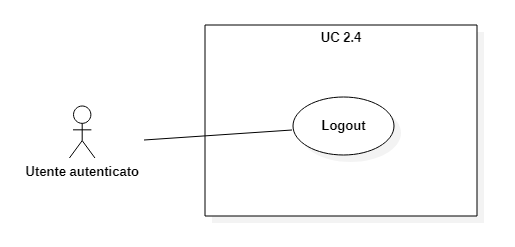
\includegraphics[scale = 0.7]{components/img/UC2_4.png}
    \caption{UC2.4 - Logout}
\end{figure}
\begin{itemize}
\item \textbf{Attore Primario:} Utente autenticato;
\item \textbf{Precondizione:} L'utente vuole effettuare il logout;
\item \textbf{Postcondizione:} L'utente ha effettuato il logout e non è più riconoscibile all'interno dell'applicazione;
\item \textbf{Scenario principale:}
    \begin{enumerate}
    \item L'utente vuole effettuare il logout;
    \item L'utente ha effettuato il logout;
    \item Tutti i file che l'utente in precedenza sincronizzava non vengono più sincronizzati con il server.
    \end{enumerate}
\end{itemize}
